\chapter{实验结果}
\label{cha:china}

在第一阶段的实验中,笔者完成了视差生成网络的loss函数编写和一部分实验,并在KITTI数据集上尝试性的进行了训练。
并且使用KITTI数据集上训好的模型在真实环境下进行了测试,KITTI数据集中测试图片效果如图~\ref{fig:kitti_res}:

\begin{figure}
\begin{subfigure}{1.\textwidth}
  \centering
  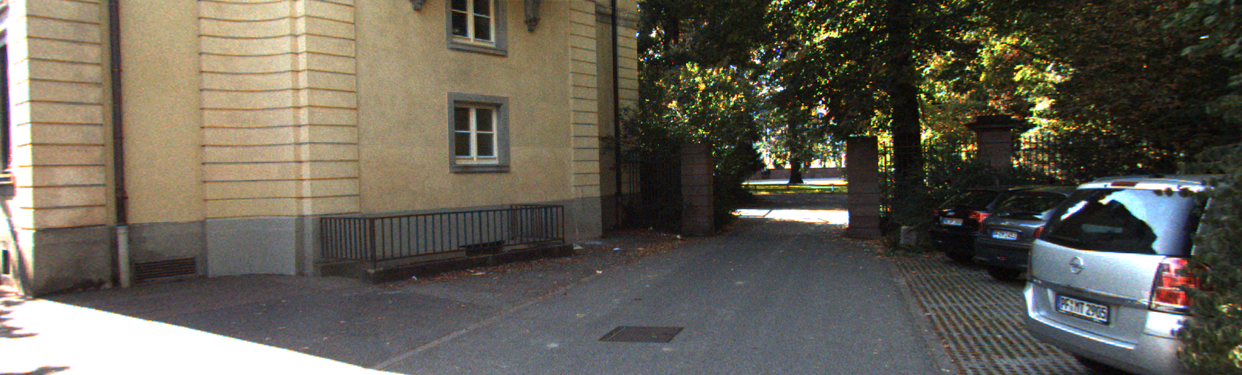
\includegraphics[width=.8\linewidth]{kitti_origin.png}
  \caption{KITTI测试集中的原图}
\end{subfigure}%

\begin{subfigure}{1.\textwidth}
  \centering
  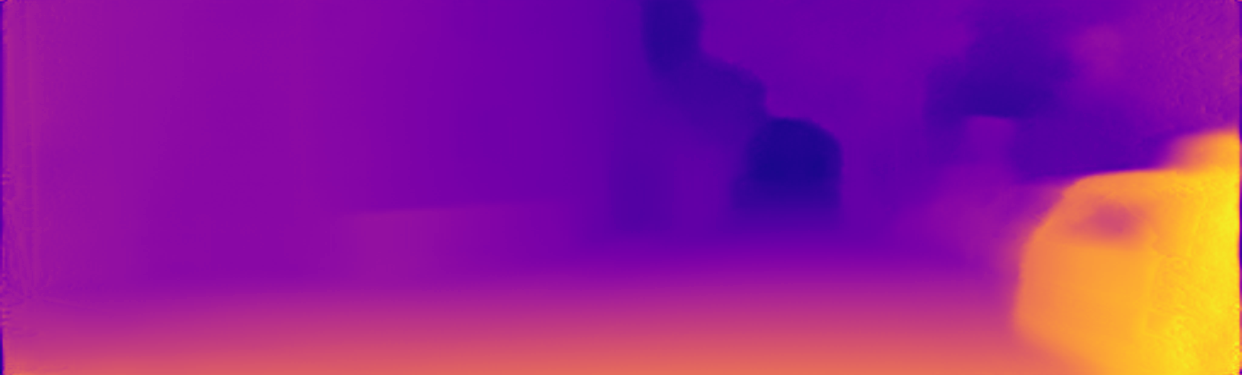
\includegraphics[width=.8\linewidth]{kitti_disp.png}
  \caption{模型生成的视差图}
\end{subfigure}
\caption{KITTI数据集中视差网络测试结果}
\label{fig:kitti_res}
\end{figure}

我们自己采集的数据测试效果如图~\ref{fig:ours_res}:


\begin{figure}
\begin{subfigure}{.5\textwidth}
  \centering
  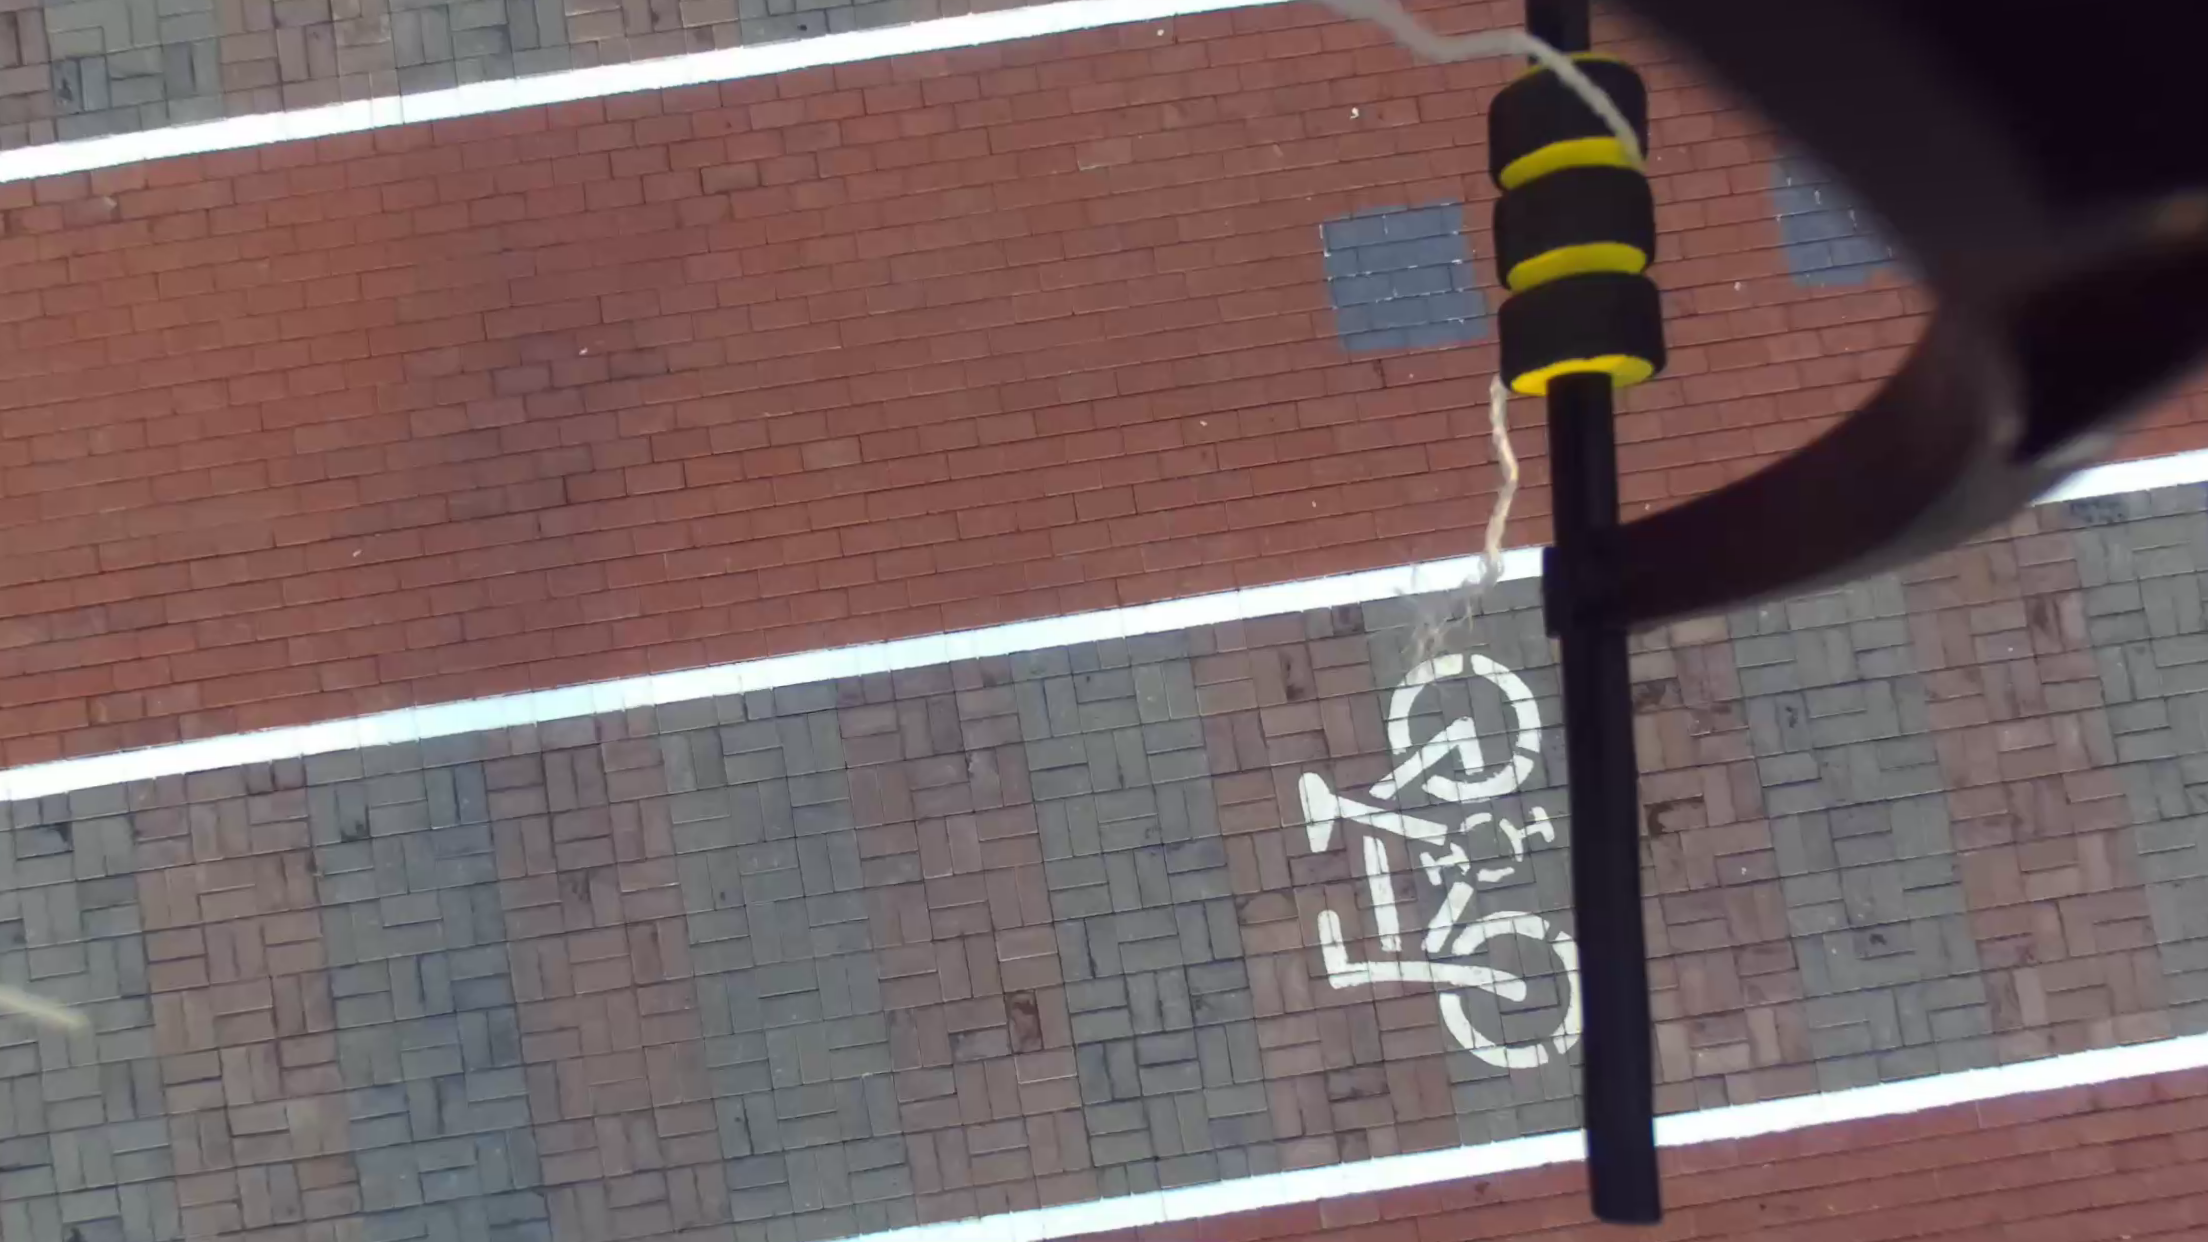
\includegraphics[width=.8\linewidth]{ours_origin.png}
  \caption{无人机采集的原图}
\end{subfigure}%
\begin{subfigure}{.5\textwidth}
  \centering
  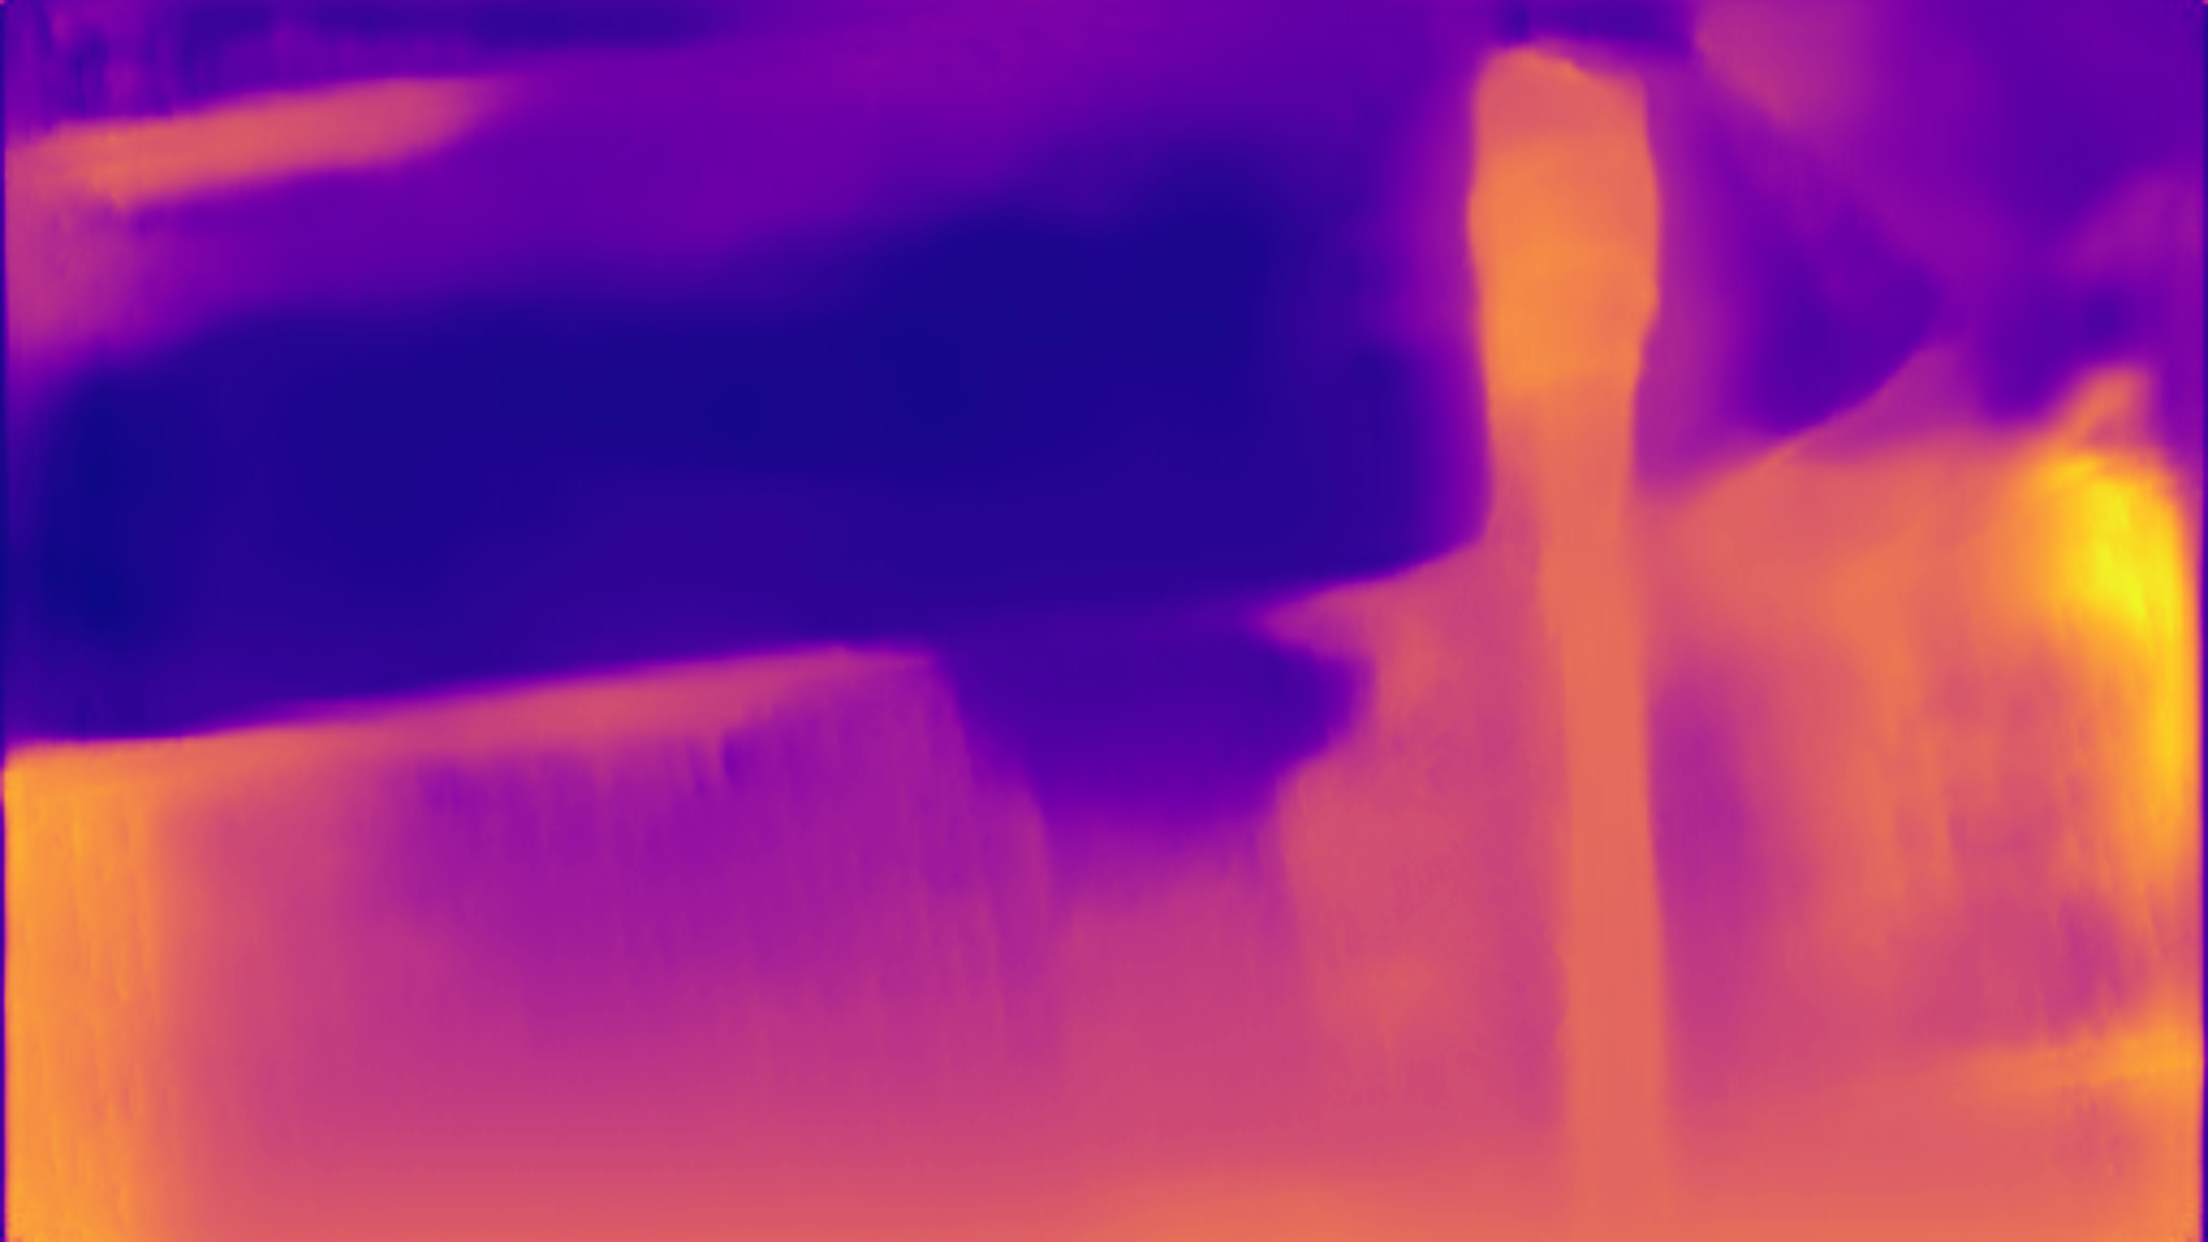
\includegraphics[width=.8\linewidth]{ours_disp.png}
  \caption{模型生成的视差图}
\end{subfigure}
\caption{ 无人机采集数据中视差网络测试结果}
\label{fig:kitti_res}
\end{figure}

可以看到,虽然没有groundtruth做对比,但是视差网络产生的结果用肉眼观看大致上是符合我们对距离的直觉的。
并且模型在KITTI上测试的结果要明显好于无人机拍摄的图片。笔者分析原因有二:一方面,视差网络在自己见过的
场景下有好的表现是可以理解的;另一方面,无人机拍摄的场景中,地面有明显的纹理,这在单目情况下对模型是异常
巨大的挑战。

在接下来的实验中,我们也许可以考虑使用无人机拍摄的场景对模型进行fine tune,并且想办法对地面纹理设置一些
约束,以配合后续的位姿估计网络的到较好的估计结果
